\documentclass[12pt,twoside,a4paper,polish]{report}
\usepackage[T1]{fontenc}
\usepackage{babel}

\usepackage[utf8]{inputenc} % https://tex.stackexchange.com/a/44699

% \usepackage{indentfirst}

\renewcommand{\thechapter}{\arabic{chapter}.}
\renewcommand{\thesection}{\thechapter\arabic{section}.}
\renewcommand{\thesubsection}{\thesection\arabic{subsection}.}

\setlength\parindent{1.25cm}

\setcounter{page}{3}

\usepackage[vmargin=2.5cm,lmargin=3cm,rmargin=2.5cm]{geometry}

\usepackage{fancyhdr}
\pagestyle{fancy}
\fancyhf{}
\fancyheadoffset{0cm}
\renewcommand{\headrulewidth}{0pt}
\renewcommand{\footrulewidth}{0pt}
\fancyhead[LO,RE]{\thepage}
\fancypagestyle{plain}{\fancyhf{}\fancyhead[LO,RE]{\thepage}}

\usepackage{helvet}
\renewcommand{\familydefault}{\sfdefault}

\linespread{1.5}

% https://texfaq.org/FAQ-run-fn-nos
\usepackage{chngcntr}
\counterwithout*{footnote}{chapter}

% \renewcommand{\theequation}{\arabic{equation}}

% TODO: https://tex.stackexchange.com/a/246285

\title{Web browsers and Internet-connected devices digital fingerprinting methods - challenges and solutions}
\author{Artur Wolff}
\date{February 2021}

\begin{document}
\chapter*{Wstęp}
\chapter*{Wstęp}

\tableofcontents
\chapter{Wprowadzenie do fingerprintingu}

\section{Podstawowe pojęcia}

\subsection{Nomenklatura używana w tej pracy}
Pisząc o odcisku palca użyto (także w tytule pracy) ogólnie przyjętego skrótu
myślowego, oznaczającego odbitkę linii papilarnych, czyli formę językową
uznawaną za poprawną przez specjalistów od daktyloskopii.

Użycie formy językowej ,,odcisk palca'' w terminie ,,cyfrowy odcisk palca'' ma
wiele sensu. Jeszcze bez zdefiniowania tego specjalistycznego terminu, możemy
domyślić się, co oznacza. Oczywiście wynika to z faktu, że cyfrowy odcisk palca
i analogowy odcisk palca są ze sobą w pewien sposób powiązane (koncepcja
cyfrowego odcisku palca czerpie z wartości wynikających ze stosowania odbitek
ludzkich linii papilarnych w dziedzinie kryminalistyki).

Angielskie słowo ,,fingerprint'' tłumaczy się jako odcisk palca, jednakże w
zagranicznych publikacjach dotyczących cyfrowego odcisku palca rzadko występuje
termin ,,digital fingerprint''. Kontekst użycia jest na tyle wyraźny, że użycie
samego ,,fingerprint'' jest wystarczające.

Zachodnie nazewnictwo ma tę przewagę, że jest zdecydowanie bardziej kompaktowe.
Także w przypadku słowotwórczego zabiegu \emph{fingerprinting}, oznaczającego
czynność; szukając polskiego odpowienika musielibyśmy sięgnąć po ,,cyfrowe
znakowanie''. Z uwagi na tę kompaktowość i łatwość użycia, w pracy preferowane
będzie użycie oryginalnej nomenklatury.

\subsection{Definicje}
W kolejnych punktach zawarto najważniejsze definicje i powiązane pojęcia, które
będą używane w przeciągu całej pracy.

\subsubsection{Fingerprint}
Wektor cech pozwalający zidentyfikować dowolny zbiór danych.

Aby fingerprint pełnił praktyczną funkcję identyfikacyjną, tak jak odbitka
ludzkich linii papilarnych pełni praktyczną funkcję identyfikacyjną, często
stosuje się algorytm, który kojarzy wektor cech z określonej długości (zwykle
krótkim) ciągiem bajtów (identyfikatorem; można go także rozumieć jako
etykieta). Takim algorytmem może być na przykład wysokiej wydajności funkcja
skrótu (niekoniecznie zdatna do zastosowań kryptograficznych---na przykład
MurmurHash). W niektórych źródłach można także spotkać się z taką definicją, że
fingerprint to już sam wynik wyżej wspomnianego algorytmu. Taka definicja nie
zmienia istoty fingerprintu, ale jest zdecydowanie mniej przydatna w kontekście
fingerprintingu urządzeń podłączonych do Internetu i przeglądarek internetowych,
czego dotyczy niniejsza praca.

\subsubsection{Fingerprint urządzenia podłączonego do Internetu}
Wektor cech pozwalający zidentyfikować urządzenie podłączone do Internetu.

\subsubsection{Instalacja przeglądarki internetowej}
Instalacja na konkretnym urządzeniu. W przypadku zmiany ustawień, konfiguracji i
liczby pluginów oraz aktualizacji przeglądarki, instalacja przeglądarki
pozostaje ciągle tą samą instalacją.

\subsubsection{Fingerprint przeglądarki internetowej}
Wektor cech pozwalający zidentyfikować instalację przeglądarki internetowej.

\subsection{Właściwości fingerprintu}
Ludzkie linie papilarne są na ogół niepowtarzalne, niezmienne i nieusuwalne. Z
wartości wynikających ze stosowania ich odbitek w swojej dziedzinie badawczej
czerpie (także etymologicznie) koncepcja fingerprintu i dlatego też fingerprint
z dobrze dobranymi cechami będzie odzwierciedlać podobne właściwości.

W przypadku fingerprintingu urządzeń podłączonych do Internetu i przeglądarek
internetowych najważniejszymi ich właściwościami są unikalność / różnorodność
(niepowtarzalność) oraz stabilność (niezmienność), przy czym zwiększenie
unikalności lub stabilności ma najczęściej negatywny wpływ na drugi parametr.

Jedną ze stosowanych\footnote{Metrykę tę stosowało na przykład badanie ,,How
	Unique Is Your Web Browser?'' Electronic Frontier Foundation; w momencie
pisania pracy jedno z największych badań tego typu.} metod pomiaru unikalności
fingerprintu urządzeń i przeglądarek jest entropia Shannona.

\subsubsection{Entropia Shannona}
Wartość entropii można rozumieć jako liczbę pytań binarnych potrzebnych do
sklasyfikowania losowo wybranego elementu z danego zbioru. Zatem entropia
Shannona zbioru \(D\) z etykietami \(\{l_{0}, l_{1}, \dots, l_{n - 1}\}\) wyraża
się wzorem \[H(D) = -{\sum_{i = 0}^{n - 1}{p(l_{i})\log_{2}{p(l_{i})}}}\] gdzie
\(p(l_{i})\) to wyrażona ułamkiem częstość \(x \in D\) mającego etykietę
\(l_{i}\). W przypadku w którym każda etykieta występuje tak samo często
entropia ma wartość maksymalną równą \(\log_{2}{n}\).

\paragraph{Przykład}
Jeśli zbiór fingerprintów przeglądarek internetowych ma \(32\) bity entropii, to
w przypadku losowego wyboru jednego z nich oczekujemy, że w najlepszym przypadku
tylko \(1\) na \(4294967295\) przeglądarek będzie miała taki sam fingerprint.

\pagebreak

\subsubsection{Stabilność}
W przypadku dodania kolejnej cechy do wektora cech, identyfikującego urządzenie
lub przeglądarkę, zwykle zwiększy to entropię, ale także zmniejszy stabilność
fingerprintu. Dzieje się tak ponieważ jest to kolejna rzecz, która może zmienić
się w czasie. Jeśli jedną z cech wejściowych jest wersja oprogramowania
urządzenia lub wersja przeglądarki (która zwykle zmienia się parę razy w ciągu
roku), to kolejne fingerprinty mogą odbiegać od siebie i naiwny klasyfikator,
korzystający z algorytmu fingerprintingowego reagującego na najmniejsze zmiany
(na przykład funkcja skrótu), mógłby nadać takiemu urządzeniu/przeglądarce
kolejną etykietę, zamiast potraktowania jej jako poprzednio widzianą instalację.

\section{Fingerprinting a Internet} % https://sjp.pwn.pl/poradnia/haslo/;228
Aby lepiej zrozumieć istotę fingerprintu i motywację stojącą za stosowaniem
fingerprintingu w kontekście urządzeń podłączonych do Internetu oraz
przeglądarek internetowych, wspominając o różnych innych obszarach przetwarzania
komputerowego w których wykorzystywany jest fingerprinting w stosownych mu
celach, kolejne punkty posłużą jako referencja (także historyczna).

\subsection{Początki Internetu}
Początek Internetu jaki znamy obecnie, to początek stworzonej w 1969 roku na
potrzeby amerykańskiego wojska sieci ARPANET. ARPANET była implementacją
koncepcji rozproszonych sieci cyfrowych transmisji danych Paula Barana z 1962
roku. Na samym początku swojego istnienia, Internet wykorzystywany był do tego
aby rozpraszać obliczenia pomiędzy wiele komputerów---w tym wypadku chodziło o
superkomputery znajdujące się w innych ośrodkach badawczych (ARPANET powstało na
Uniwersytecie Kalifornijskim w Los Angeles). W tym samym okresie powstawały inne
globalne sieci komputerowe, zapoczątkowane zwykle w innym celu (na przykład
komunikacyjnym, rozrywkowym), które później połączono z ARPANET. Badacze
historii Internetu wskazują na fakt, iż gwałtowny rozwój Internetu zawdzięcza
się właśnie komunikacyjnemu i rozrywkowemu aspektowi konkurencyjnych sieci.

\begin{figure}
	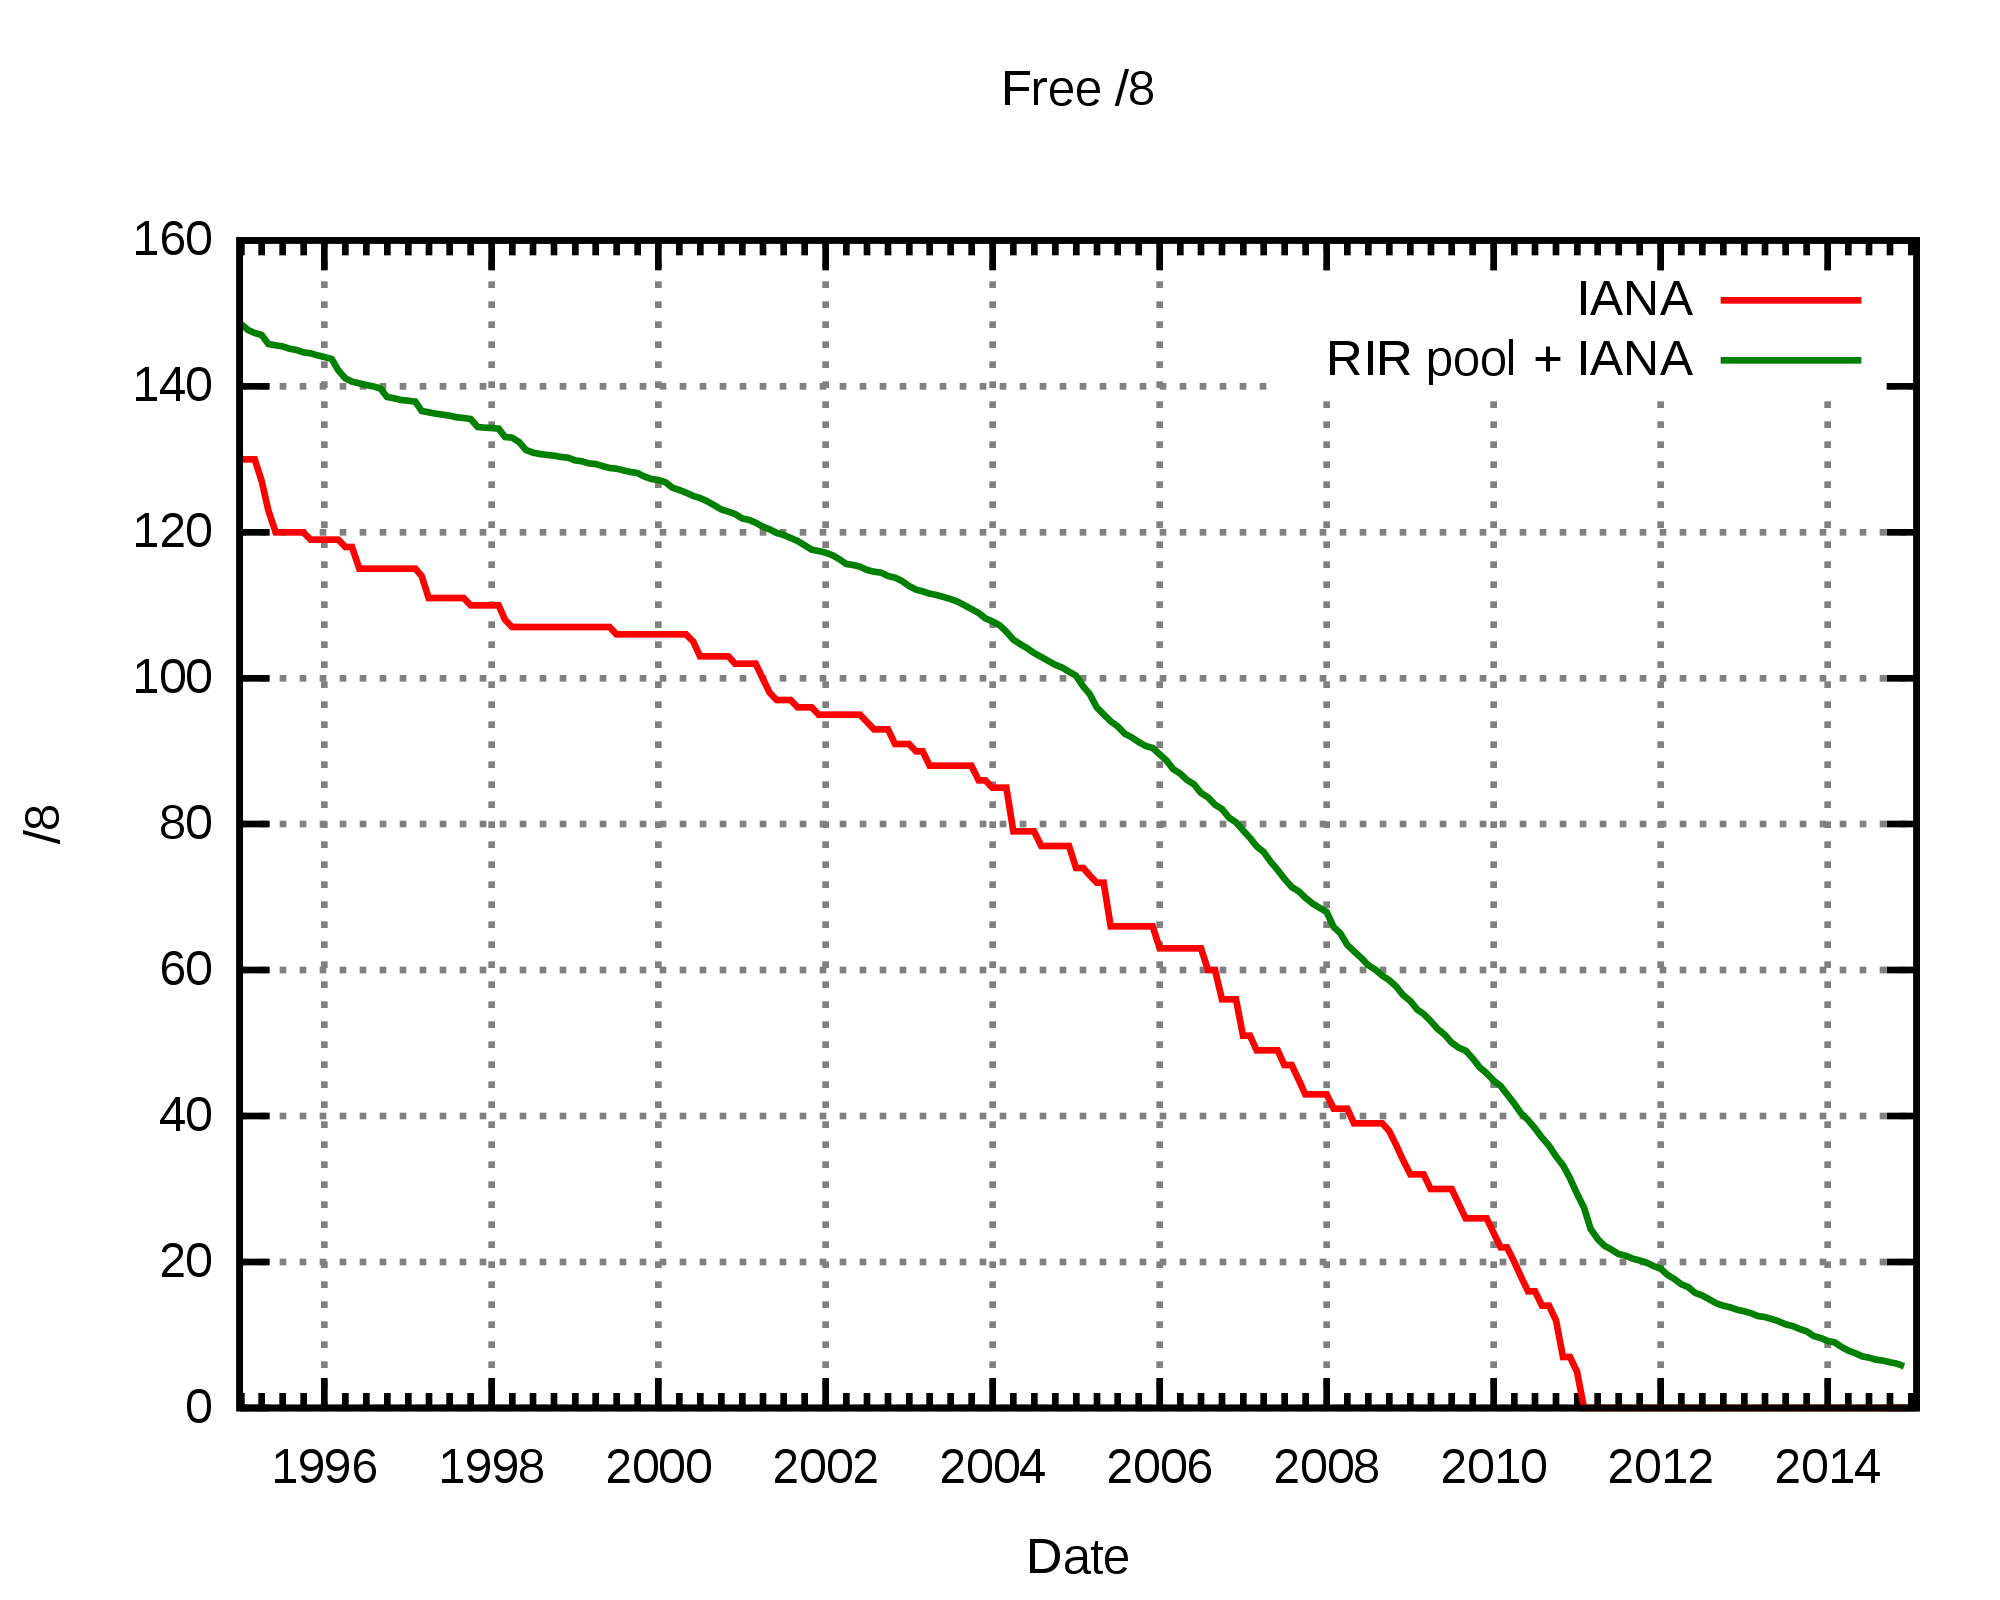
\includegraphics[width=\textwidth,height=\textheight,keepaspectratio]{img/01.png}
	\source{http://www.opte.org/maps/ (odwrócono kolory w celu zaoszczędzenia tuszu)}
	\caption{Mapa Internetu z 16 stycznia 2005 roku.}
\end{figure}

\subsection{Założenia funkcjonowania Internetu i ich realizacja}
Po tym jak w 1989 Tim Bernes-Lee oraz Robert Cailliau utworzyli projekt sieci
dokumentów hipertekstowych, czyli tego, co obecnie znamy jako World Wide Web i
strony internetowe, osoby prywatne oraz instytuje komercyjne zaczęły dostrzegać
korzyści z użytkowania Internetu, a szczególnie z wykorzystania go jako medium
reklamy i sprzedaży. Zniesienie zakazu wykorzystywania Internetu do celów
komercyjnych w 1991 roku zakończyło chwilę w której Internet był medium
naukowego dyskursu i zapoczątkowało okres istnienia Internetu dla mas, który
trwa do dziś.

\subsubsection{Początki śledzenia użytkowników Internetu}
\dots

\subsubsection{Perspektywa techniczna}
Podstawą struktury obecnego Internetu jest model TCP/IP i konceptualnie składa
się ze współpracujących ze sobą 4 warstw:
\begin{enumerate}
	\item dostępu do sieci
	\item kontroli transportu
	\item Internetu
	\item aplikacji
\end{enumerate}
W najwyższej z warstw, czyli warstwie aplikacji działają takie usługi jak
przeglądarka czy serwer WWW. To najbardziej interesująca warstwa z perspektywy
niniejszej pracy, ale fingerprinting urządzeń podłączonych do Internetu może
odbywać się także w niższych warstwach. % TODO Elaborate?

\section{Fingerprinting w branży komputerowej}
Fingerprinting to technika wykorzystywana w wielu obszarach w dyscyplinie
informatyki; fingerprinting urządzeń podłączonych do Internetu i przeglądarek
internetowych to tylko pewien wycinek zastosowań tej koncepcji. O ile podane na
początku tego rozdziału definicje ujmują fingerprint w sposób ogólny i także
taki, który pokrywa się z definicjami, które można znaleźć w publikacjach
dotyczących fingerprintingu urządzeń i przeglądarek, to definicje dotyczące
zastosowań fingerprintu innych bytów mogą być bardziej specyficzne czy też mogą
zwracać większą uwagę na inne właściwości, charakterystyczne dla stosownych
zastosowań. Kolejne punkty służą jako referencja do ukazania jak szeroko
wykorzystywana jest omawiana koncepcja.

\subsection{Fingerprinting audio, wideo i algorytmy ACR}

\subsection{Fingerprinting klucza publicznego}

\listoffigures
\listoftables
\end{document}
